\documentclass[12pt]{article}
\usepackage[utf8]{inputenc}
\usepackage{amsmath}
\usepackage{graphicx}
\usepackage{listings} % for source code inserts
\title{CS 470 Spring 2011 \\
     Project 2}
\author{Colby Blair}
\date{Due March 25th, 2011}
\begin{document}
\maketitle

\begin{abstract}
In artificial intelligence (AI), we can create and measure intelligent agents in
games. Games are simplified situations from real life, and the logistics of 
games are more tractable for AI. This report uses Connect 4 to attempt creation
of intelligent agents. They will use different algorithms, some deterministic 
and some semi-random. As the searches increase in complexity, and 
semi-randomness increases, game play becomes more advanced. It also seems
more intelligent. It is still, however, deterministic.

No algorithm here is a clear winner. Some are always worse than others, but some play better in certain 
condions, and fall apart in others. These conditions are complex, too. The general winning family of 
algorithms are alpha beta pruning. These algorithms, once finding a sure win or lose on a potential move,
don't waste more time exploring. After thinking about the problem, they seem like the best choice, although
they do not always win.
\end{abstract}

\pagebreak

\tableofcontents
\listoffigures

\pagebreak


\section{Introduction}

\begin{figure}[h]
        \begin{center}
		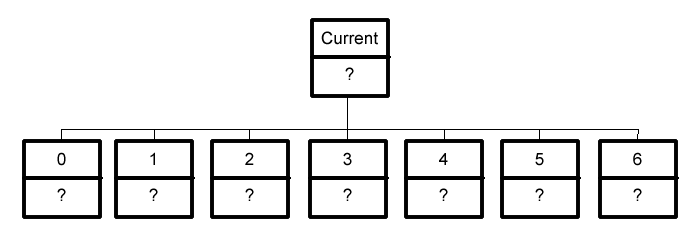
\includegraphics[width=100mm]{report_images/mm_init.png}
                	\caption{Most games in Connect 4. Top values are potential column moves, 
				bottom (?) are how good the moves would be. }
                	\label{mm_init}
        \end{center}
\end{figure}

In Connect 4, almost everytime a player considers a move, the player havs 7 choices. Humans usually look a 
few moves ahead, consider future gameplay, and make estimations on what are good moves. If the game gets
too complex and future move impacts are unclear, humans make general estimations on what patterns or
groups of pieces seem like good groupings.

The intelligent agents in this report will also try all these things. Although they are not really what humans 
would define as intelligent (see 'Turing Test'), they are able to perform complex operations usually past the ability of a human. Their job is to assign real numbers in place of the '?'s in Figure \ref{mm_init}. As this report will show, this becomes a big challenge.

As their gameplay becomes more deterministic off of the present conditions, seem more
random, or just seem more complex in general, the agents seem more intelligent. They are completely 
deterministic, though, and depending on your philisophy, may be disqualified from being intelligent at all.

One observation is that the algorithms never learn from previous moves. In the author's opinion, this is the disqualifying characteristic of their intelligence. If they did learn, they would have the most basic form of 
intelligent, but would arguably be intelligence. This makes broader claims on philosophies, but is the author's
claim.


\section{Algorithm Concepts}

\subsection{Min-Max}

\begin{figure}[h]
        \begin{center}
		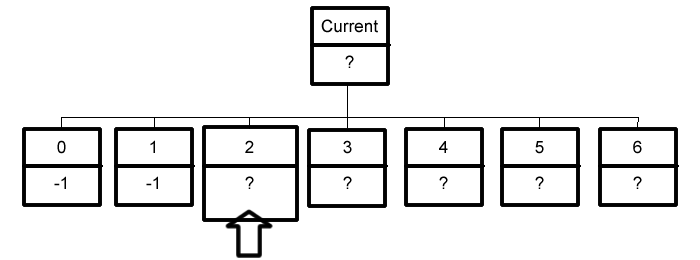
\includegraphics[width=100mm]{report_images/mm_top.png}
                	\caption{MinMax assigning values to potential moves at depth 1. }
                	\label{mm_top}
        \end{center}
\end{figure}

Min-Max algorithms are the first step in the direction of trying to quantify how good a potential move is.
First, it is the intellgent agent's move. This algorithm makes a copy of the current game, and runs a simulation. Then it looks at the potential moves (Figure \ref{mm_top}), and says 'What if I move here?' If the 
answer is 'I will win', then that move gets a 1 value. If the answer is 'I will lose', the move gets a -1 value. 
If the answer is 'I neither win nor lose', then the algoritm makes the move in its simulation, and continues to
the next step.

\begin{figure}[h]
        \begin{center}
		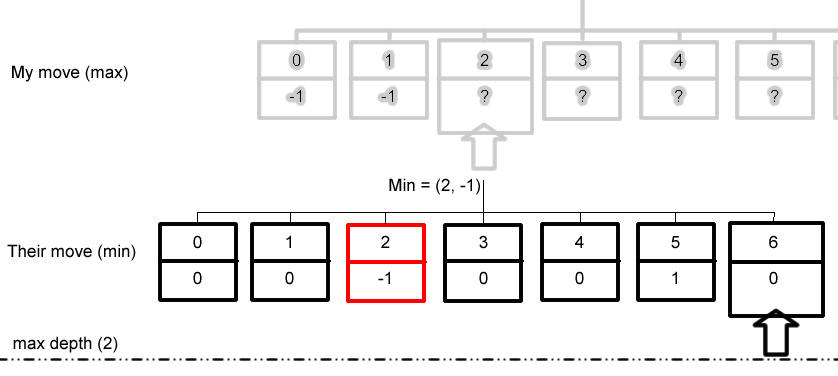
\includegraphics[width=100mm]{report_images/mm_d2.png}
                	\caption{MinMax assigning values to potential moves at depth 2.}
                	\label{mm_d2}
        \end{center}
\end{figure}

The next step (Figure \ref{mm_d2}), after making the potential move, is to evaluate what the opponent's options are (the opponent is the live human). For every move, this algorithm asks 'What if the opponent moves here?'. If the answer is 'They will will', the move gets a -1 value. If the answer is 'They will lose', the move gets a 1 value. If the answere is 'They will neither win nor lose', then the algorithm makes the move in its simulation, and looks at it the same way as it looked at the first branch above.

With is scheme, this algorithm says -1 values will make me lose, 1 values will make me win. In Figure \ref{mm_d2}, there are 0 values. These are where the algorithm thinks 'Neither me nor my opponent will win or lose, and I have gone as deep as I can go'. Maximum depth is important, because every level of depth that
is added, search time increases exponentially (as this report will later show).

\begin{figure}[h]
        \begin{center}
		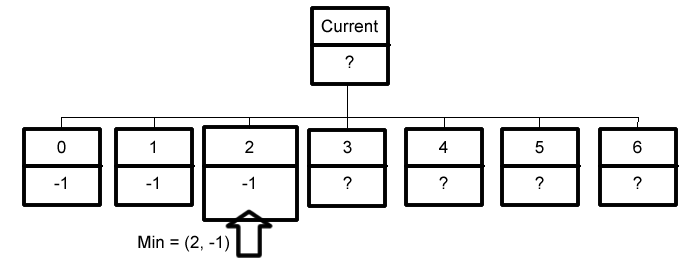
\includegraphics[width=100mm]{report_images/mm_reduce.png}
                	\caption{MinMax setting the value from depth 2, Figure \ref{mm_d2}.}
                	\label{mm_reduce}
        \end{center}
\end{figure}

The min-max part of the algorithm is this: if the algorithm is considering the opponent's ('their') potential
moves, it must return the minumum back up the tree (Figure \ref{mm_reduce}). If it is considering the agent's ('my') moves, it must return the maximum. 

This algorithm essentially says that if the algorithm is considering the opponents moves, the
opponent will always pick the move that hurts the most (minimum). If it is considering the agent's moves,
the agent will always take the move that helps the most (maximum). Sure win paths come to the top, and sure lose paths are avoided unless there is no choice.

The advantage at the beginning of the game is none, but as the board fills up, more wins and loses are possible, and more pruning occurs.

\pagebreak

The pseudo code for the algorithm choosing the best move to play is as follows:

\scriptsize
\begin{lstlisting}
minmax(self,c4_orig,depth):
 for i in 0,columns:
  if potgames[i].play_piece(i):
   if depth < maxdepth and not potgames[i].is_winner():
    potgames[i].hval = minmax(potgames[i],depth + 1)
   else:
    potgames[i].hval = h2(potgames[i])
  else: #if not potgame[i].play_piece(i)
   if turn  == black:
    potgames[i].hval = -2
   elif turn == red:
    potgames[i].hval = 2
 if turn == black:
  return max(potgames)
 else if turn == red:
  return min(potgames)
\end{lstlisting}
\normalsize

Future algorithms will also share this general structure.


\subsection{Alpha-Beta Pruning}

\begin{figure}[h]
        \begin{center}
		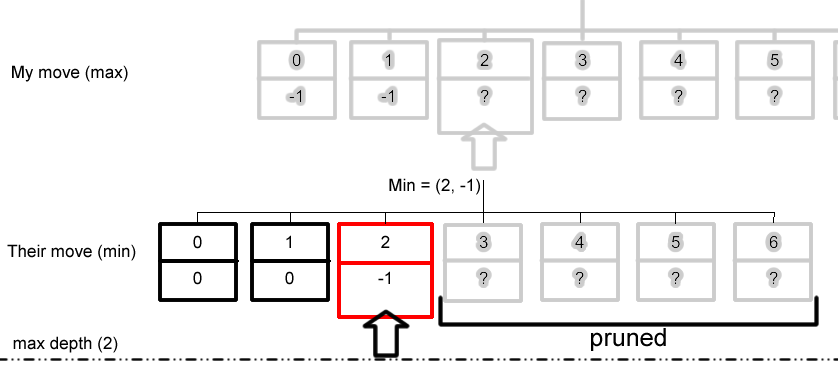
\includegraphics[width=100mm]{report_images/ab_d2.png}
                	\caption{Alpha-Beta search at depth 2.}
                	\label{ab_d2}
        \end{center}
\end{figure}

The Alpha-Beta Pruning algorithm uses the Min-Max algorithm, making some improvements. Consider again Figure \ref{mm_d2}, and compare with Figure \ref{ab_d2}. When considering move 2 at depth 2, the algorithm get set a -1 values. This will be the most negative result. But the algorithm unneccesarily searches the rest of the moves in Figure \ref{mm_d2}. If the max depth was greater, the algorithm would waste even more time
searching deeper branches.

Alpha-Beta Pruning basically says that when in a minumum branch (opponent move), if the absolute minumum (-1) score is set (beta), return it up the tree immediately. Simularly, when in a maximum branch (my 
move),  if the absolute maximum (1) score is set (alpha), return it up the tree immediately. Figure \ref{ab_d2}
shows this; once -1 is set and move 2, then that value is returned up the tree.


\subsection{Alpha-Beta Pruning with Time Estimation}
With Alpha-Beta Pruning, the algorithm speeds up search time. But what if search time isn't the prime
concerm? What if the algorithm has a time limit, but we want to maximize searched branches within that time
limit? In both Min-Max and Alpha-Beta pruning, we set a static max depth, so that all searching didn't exceed
a time limit. Mainly, searching at the beginning of the game. But as game play continues, the game has less
possible moves. Possible wins and losses should increase, and pruning in general should increase. 

Alpha-Beta Pruning with Time Estimation attempts to address this. It determines a search time estimate, 
based on how late in the game (pieces played), how long in raw seconds it has taken to search one more
node down in the tree, and how many nodes are in the search tree at a new depth. If the estimated time
exceeds the maximum allowable run time, the algorithm sets the max depth, and begins the search.

This description leaves out some details and gotchas. The algorithm for determining max depth on every
turn is as follows:

\begin{tabular}{ r l }
	\(D_{max}\)			& \(= D_{T_{cutoff}}\) 						\\
						& \(\exists\) \\
						& \( T_{cuttoff} = B_{reduced}^{D} * T_{total}\)\\
						& \( T_{cuttoff} <= T_{max}\)\\
						& \(B_{reduced}  = B - ( total turns / B) \)
\end{tabular} \\

\pagebreak

This is better explained in pseudo code. The 'times\_up' function basically takes the place of 'if depth $>=$ maxdepth' in the minmax psuedo code:

\scriptsize
\begin{lstlisting}
       times_up(depth,branching_factor):
                #always allow depth 0 analysis
                if depth == 0:
                        return False
                if maxdepth == -1: #not inited
                        reduce_branching_factor = total_turns / branching_factor
                        branching_factor = branching_factor - reduce_branching_factor
                        pottime = (branching_factor ^ depth) * total_run_time
                        if (pottime >= time_limit): 
				#set max depth
                                maxdepth = depth
                                return True
                else if depth >= maxdepth:
                        return True
                #emergency time check. -1 seconds to give a little buffer
                if (self.run_time > self.time_limit - 1):
                        return True
                return False
\end{lstlisting}
\normalsize

The time estimate allows the Alpha-Beta test to have a low depth in the beginning of the game, but as the 
game goes on and more pieces are played, the depth is extended. This is possible because more of the tree
can pruned, and searches are generally quicker.

There are instances where some branches of the tree are not well prunable. If the algorithm chooses these
branches first, it may go too deep and run out of time to check the other branches. In this case, once time is low, it returns up the tree, checks the 0 depth (depth 1 in the figures) for any moves than need to be blocked,
and basically reverts to very basic game play. 


\subsection{Probabilities at Low Depth}
\label{sec:prob_lowd}
This algorithm is different from the rest, in that it does't really search a decision tree at all. Instead, it only
considers the first level of the tree (depth 1). For all 7 potential boards, the evaluation function calculates a
probability of a win. This is explained more in Section \ref{sec:h1}, H1.

Most of the processing is done in the evaluation function, H1. This makes it not very useful for shotgun or
deep searching algorithms on the tree. Somewhat suprisingly, however, it performs very well compared to 
the most advanced search algorithms. It also takes a fraction of the time.

\pagebreak


\subsection{Evaluation Functions}

\subsubsection{H2}
All algorithms except the Probabilities at Low Depth algorithm (Section \ref{sec:prob_lowd}) use this evaluation function. It works as follows:
\begin{itemize}
	\item if winner is detected:
	\begin{itemize}
		\item if turn == mine
		\begin{itemize}
			\item return 1
		\end{itemize}
		\item else
		\begin{itemize}
			\item return -1
		\end{itemize}
	\end{itemize}
	\item else
	\begin{itemize}
		\item return 0
	\end{itemize}
\end{itemize}

If the algorithm gets a 0 value from H2, it will process that move's sub-branches until a min or max is found,
or the max depth is reached. If the top level branch is all zeros, then a move is selected at random.

\subsubsection{H1}
\label{sec:h1}
This function is used only by Probabilities at Low Depth algorithm (Section \ref{sec:prob_lowd}). It finds the probability of a piece leading to a win, based on that newly placed piece's environment:

\begin{equation}
	P_{total} = P_{y}() + P_{x left} + P_{x right}
 \end{equation} \\

where x and y are the coordinates of the potentially dropped piece. x increases from left to right, y increases from top to bottom.

\pagebreak

\begin{itemize}
	\item if board[x][y+1] and board[x][y+2] and board[x][y + 3] are not opponents pieces
	\begin{itemize}
		\item $P_{y}() = sum(P_{piece}(x,y:y + 3)$
	\end{itemize}
	\item else
	\begin{itemize}
		\item $P_{y}() = 0$
	\end{itemize}
	\item if board[x-1][y] and board[x-2][y] and board[x-3][y] are not opponents pieces
	\begin{itemize}
		\item $P_{x left}() = sum(P_{piece}(x:x-3,y)$
	\end{itemize}
	\item else
	\begin{itemize}
		\item $P_{x left}() = 0$
	\end{itemize}
	\item if board[x+1][y] and board[x+2][y] and board[x+3][y] are not opponents pieces
	\begin{itemize}
		\item $P_{x right}() = sum(P_{piece}(x:x+3,y)$
	\end{itemize}
	\item else
	\begin{itemize}
		\item $P_{x right}() = 0$
	\end{itemize}
	\item if board[x][y] == empty
	\begin{itemize}
		\item $P_{piece}(x,y) = 1$
	\end{itemize}
	\item if board[x][y] == my piece
	\begin{itemize}
		\item $P_{piece}(x,y) = 3$
	\end{itemize}
\end{itemize}

This function basically gives probabilities on each potential move one could make. A potential win could be
to the left, to the right, and up. H1 ignores diagonals wins, although they seem to actually be included.
The probability of a future win is a sum of all the probable plays around a potentially played piece.

\pagebreak

\section{Time and Depth Comparisons}
\small
\begin{tabular}{| c | c | c |}
	\hline
	\textbf{Algorithm}	&	\textbf{Run Time} (seconds)	&	\textbf{Max Depth Reached} \\
	\hline
	Min-Max			&	7.30					&	5					\\
	\hline
	Alpha Beta Pruning	&	7.36 - $>$ 0.00			&	5					\\
	\hline
	Alpha Beta Pruning with Time Estimation	&	29.10 - $>$ 0.00	&	9		\\
	\hline
	Probabilities at Low Depth	&	.006		&	1							\\
	\hline
\end{tabular}
\normalsize


\section{Conclusion}
The algorithms have clear differences. Alpha Beta Pruning is a clear improvement over MinMax. MinMax is not
the optimal algorithm in any aspect. Alpha Beta Pruning with Time Estimation is clearly different from the rest.
Probabilities at Low Depth takes a different approach altogether. What isn't clear is which plays the best game.
Alpha Beta Pruning with Time Estimation plays very good most of the time, but will sometimes miss shallow
wins that Alpha Beta Pruning will catch. In conclusion, a hybrid of Alpha Beta Pruning with time estimation and
Probabilities at Low Depth may be a very good solution.

\section{Results}

\pagebreak

%\subsection{Min-Max}

\begin{figure}[h!]
        \begin{center}
		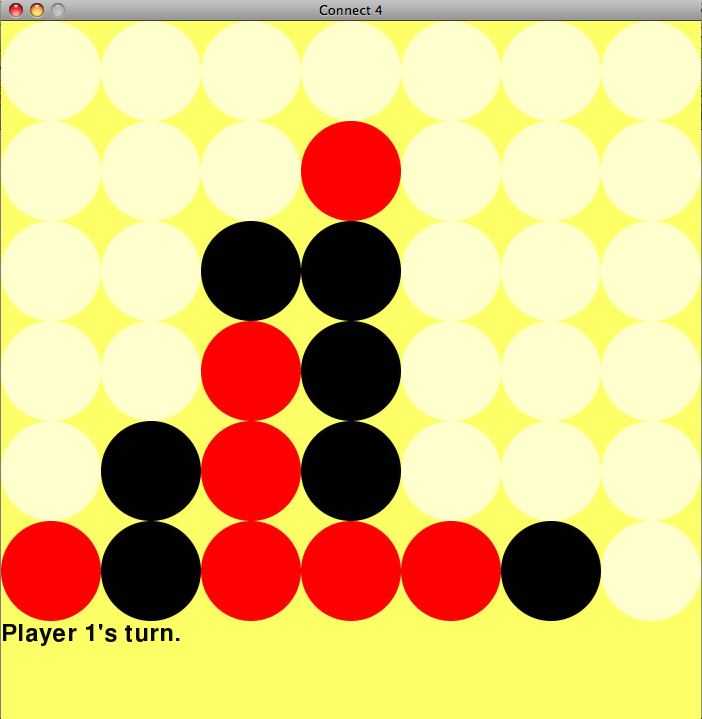
\includegraphics[width=60mm]{report_images/mm_play.png}
		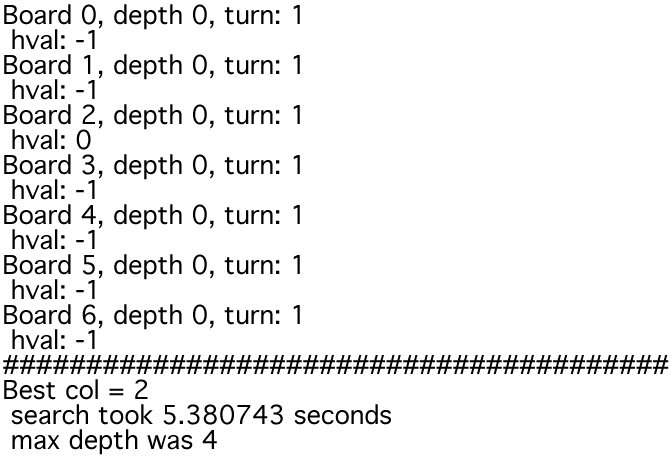
\includegraphics[width=60mm]{report_images/mm_play_text.png}
                	\caption{MinMax playing Connect 4. Last move is a block.}
                	\label{mm_play}
        \end{center}
\end{figure}


%\subsection{Alpha-Beta Pruning}

\begin{figure}[h!]
        \begin{center}
		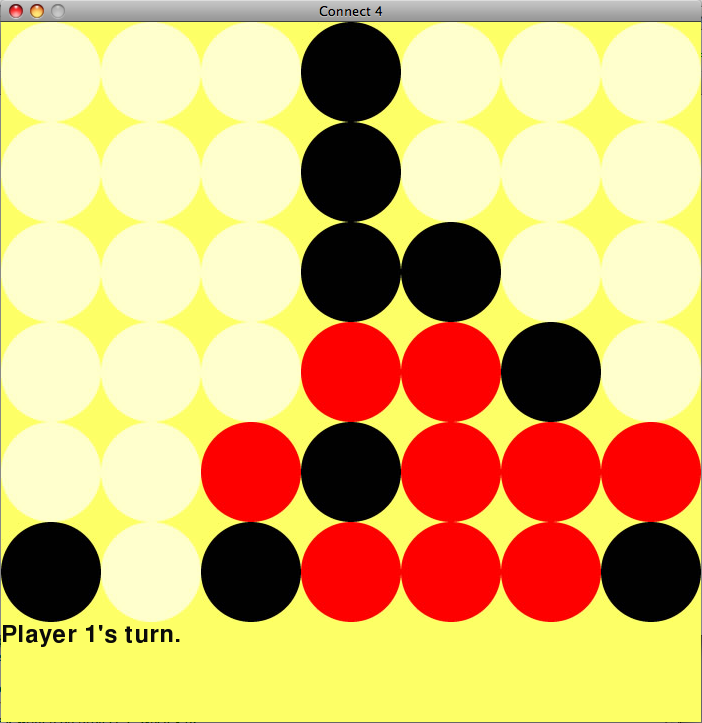
\includegraphics[width=60mm]{report_images/ab_play.png}
		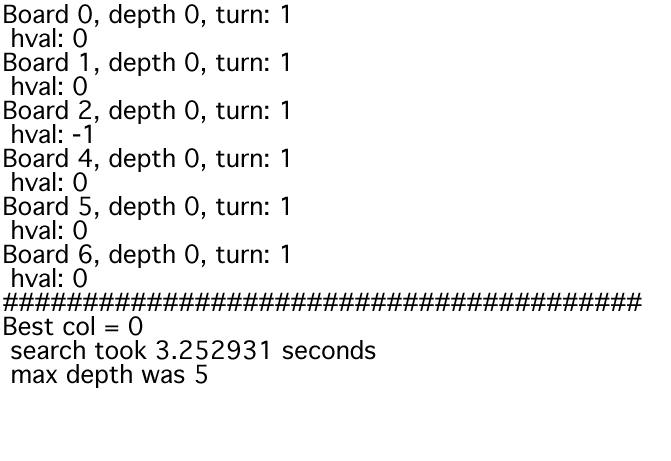
\includegraphics[width=60mm]{report_images/ab_play_text.png}
                	\caption{Alpha-Beta Connect 4. Mid game.}
                	\label{ab_play}
        \end{center}
\end{figure}


%\subsection{Alpha-Beta Pruning with Time Estimation}

\begin{figure}[h!]
        \begin{center}
		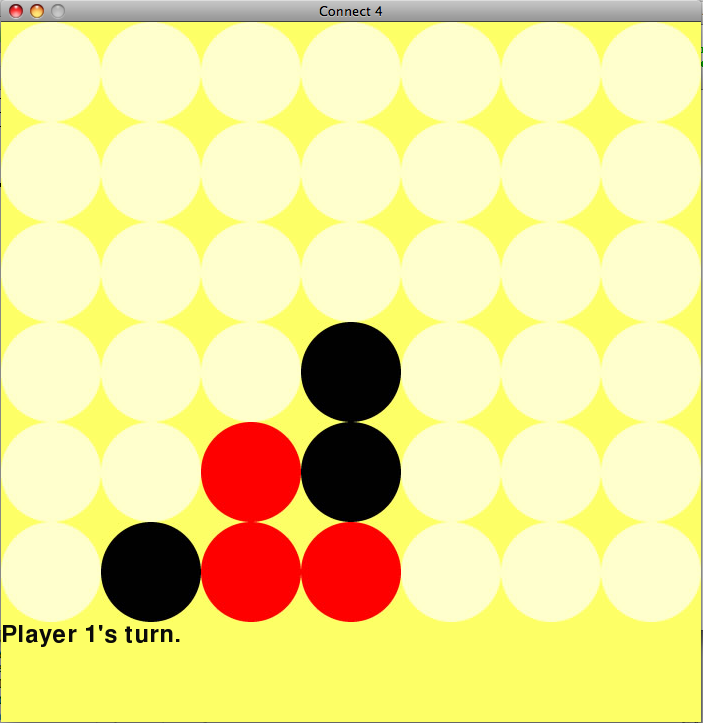
\includegraphics[width=60mm]{report_images/abt_play.png}
		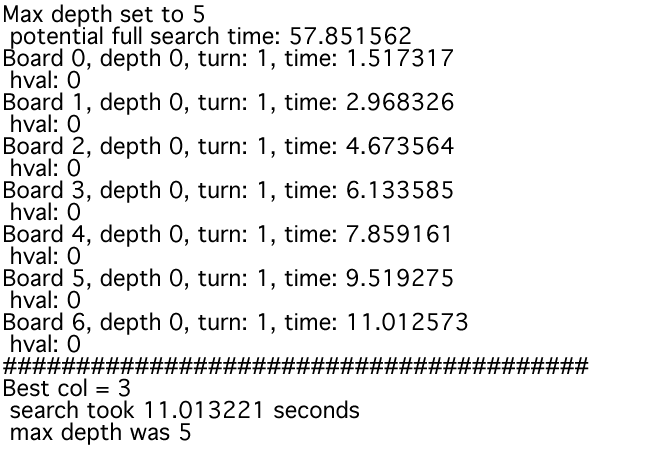
\includegraphics[width=60mm]{report_images/abt_play_text.png}
                	\caption{Alpha-Beta with Timed Estimate playing Connect 4. Beginning game.}
                	\label{abt_play}
        \end{center}
\end{figure}

\begin{figure}[h!]
        \begin{center}
		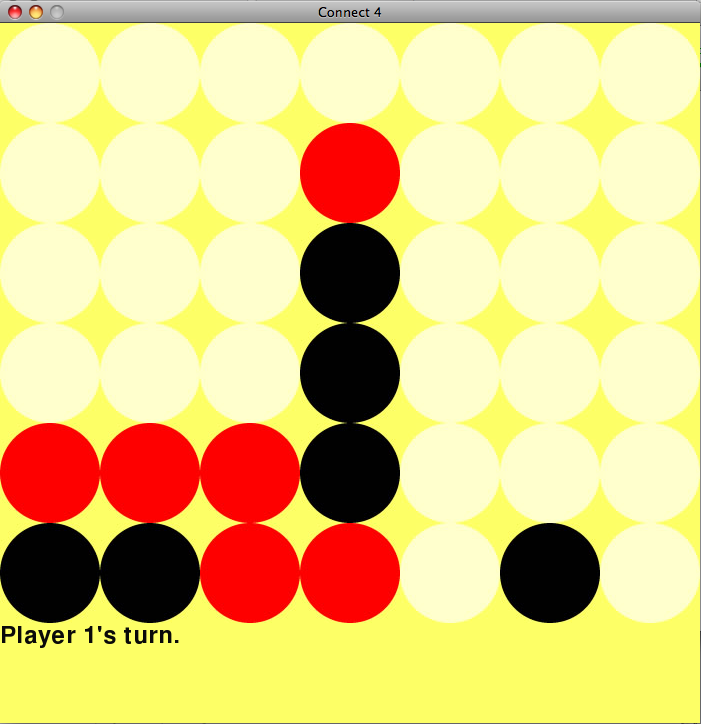
\includegraphics[width=60mm]{report_images/abt_play_mid.png}
		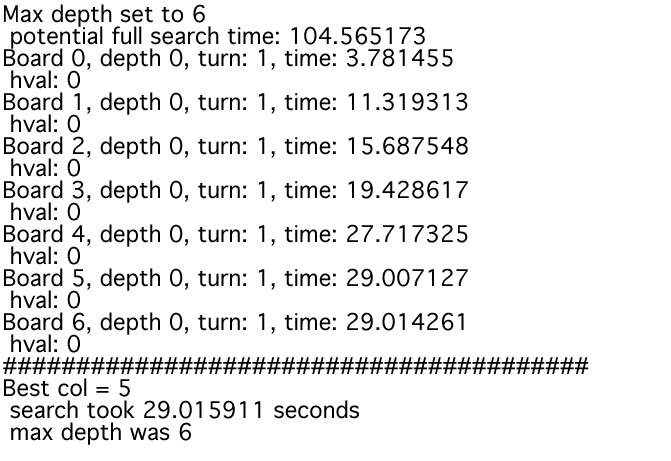
\includegraphics[width=60mm]{report_images/abt_play_mid_text.png}
                	\caption{Alpha-Beta with Timed Estimate playing Connect 4. Mid game with increased depth.}
                	\label{abt_play_mid}
        \end{center}
\end{figure}

\begin{figure}[h!]
        \begin{center}
		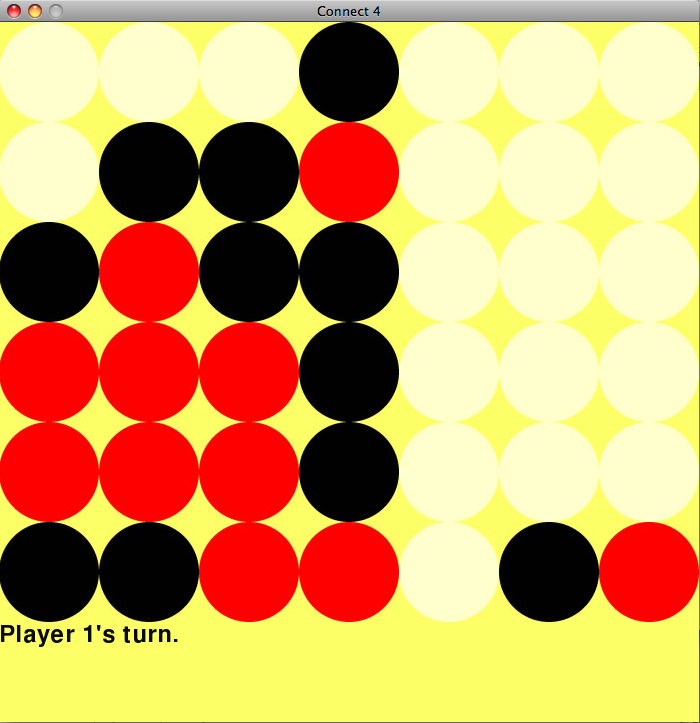
\includegraphics[width=60mm]{report_images/abt_play_det_win.png}
		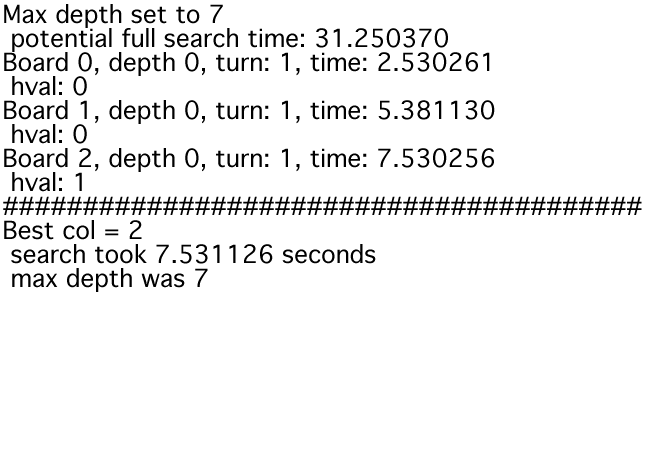
\includegraphics[width=60mm]{report_images/abt_play_det_win_text.png}
                	\caption{Alpha-Beta with Timed Estimate playing Connect 4. End of game, more depth increase, win found deep down.}
                	\label{abt_play_det_win}
        \end{center}
\end{figure}


%\subsection{Probabilities at Low Depth}
\begin{figure}[h!]
        \begin{center}
		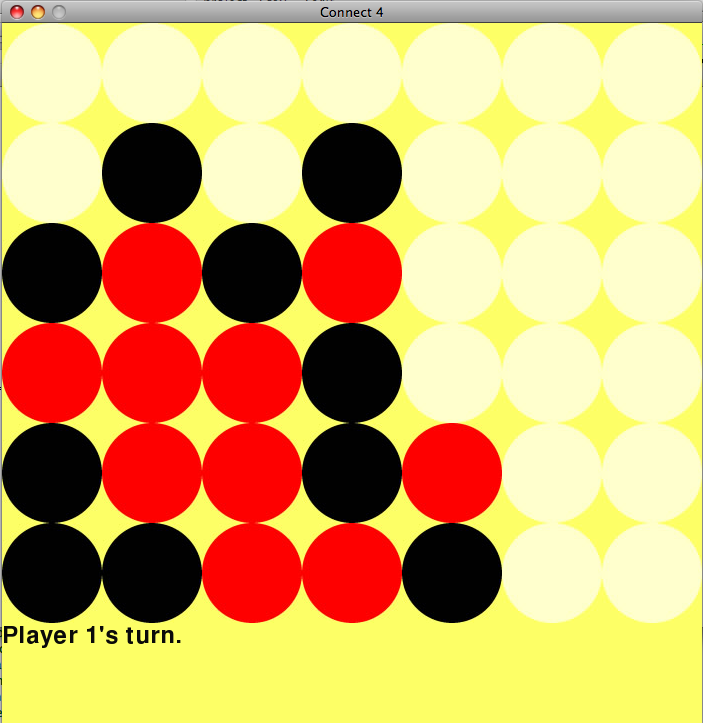
\includegraphics[width=60mm]{report_images/prob_play.png}
		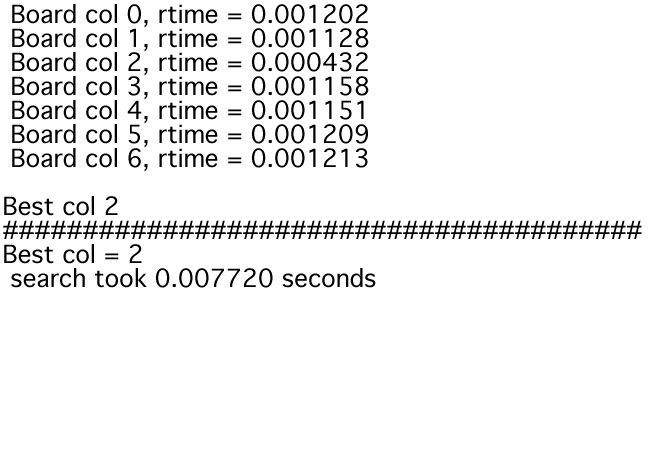
\includegraphics[width=60mm]{report_images/prob_play_text.png}
                	\caption{Probabilities at Low Depth}
                	\label{prob_play}
        \end{center}
\end{figure}


\end{document}
